Il \textit{Data Analyzer} si occupa dell'analisi dei dati raccolti dal \textit{Data Collector} al fine di generare gli allarmi che saranno poi visibili agli utenti tramite l'applicazione client. Come per il \textit{Data Collector}, si è deciso di implementare questo componente come un applicativo Python che verrà in seguito distribuito su un Raspberry Pi 4 per la sua esecuzione periodica. Si è scelto di utilizzare questo linguaggio di programmazione poiché sono disponibili numerose librerie per effettuare analisi dei dati e che verranno sfruttate per la generazione delle allerte. In particolare, si è scelto di implementare le allerte per segnalare i rischi di nebbia o brina e l'imminente arrivo di una forte perturbazione. Nella figura \ref{fig:DAFlowChart} è rappresentato il diagramma di flusso relativo al Data Analyzer. All'avvio dell'applicazione vengono inizializzate alcune strutture dati necessarie all'esecuzione degli algoritmi per l'analisi dei dati, algoritmi che sono descritti dettagliatamente in seguito. Successivamente, viene eseguito un tentativo di connessione con il DB seguendo una strategia uguale a quella utilizzata per il \textit{Data Collector}. Se la connessione viene stabilita con successo, vengono recuperati dal DB  i codici identificativi delle stazioni meteorologiche; essi saranno utilizzati successivamente per accedere ai dati da fornire in input agli algoritmi per la generazione degli allarmi. Dopodiché, viene avviato un thread per ogni zona, il quale si occuperà della generazione delle allerte maltempo tramite l'analisi dei dati relativi alla pressione atmosferica. Inoltre, vengono avviati anche i thread che si occupano di analizzare i dati di temperatura e umidità relativa al fine di creare le allerte nebbia e brina. Infine, si attende la terminazione di tutti i thread precedentemente avviati e, a join concluso, viene chiusa la connessione con il DB. Da notare che la periodicità del ciclo è di 5 minuti.

\begin{figure}[h!]
	\centering
	\includegraphics[height=590px]{./Iterazione 3/OtherFiles/FC - Data analyzer}
	\caption{Diagramma di flusso relativo all'esecuzione del componente Data Analyzer.}
	\label{fig:DAFlowChart}
\end{figure}

\clearpage

\paragraph{Generatore di allerte maltempo} 

\subparagraph{Cenni di meteorologia} Esistono due differenti approcci per prevedere l'andamento delle condizioni meteorologiche a partire dalle rilevazioni della pressione atmosferica $p_{atm}$:
\begin{itemize}
	\item \textit{generale} (analisi della $p_{atm}$ in termini assoluti): se la pressione è inferiore a \SI{1000}{\hecto\pascal}, allora è probabile che il tempo volga brutto; tale probabilità aumenta in presenza di venti meridionali e di un'umidità superiore al \SI{50}{\percent}. Se, invece, la pressione è superiore a \SI{1025}{\hecto\pascal}, allora è probabile che il tempo tenda al bello; tale probabilità aumenta in presenza di venti settentrionali e di un'umidità inferiore al \SI{60}{\percent};
	\item \textit{specifico} (analisi della $p_{atm}$ in termini di variazioni temporali): un calo di 1-\SI{2}{\hecto\pascal} in 3 ore precorre un peggioramento che si manifesta entro le prossime 24-48 ore, una diminuzione superiore a 2-\SI{3}{\hecto\pascal} in 3 ore entro le prossime 12-24 ore, mentre un calo di 5-\SI{6}{\hecto\pascal} in 3 ore sta a indicare un peggioramento imminente per di più da associare a una perturbazione violenta. 
\end{itemize}
La pressione atmosferica, inoltre, è soggetta a un andamento periodico nel corso del giorno:
\begin{itemize}
	\item primo minimo alle ore 4;
	\item primo massimo alle ore 10;
	\item secondo minimo alle ore 16;
	\item secondo massimo alle ore 22.
\end{itemize}
Pertanto, è importante innanzitutto destagionalizzare la serie storica delle misure di pressione affinché possano essere studiate le variazioni relative esclusivamente a un cambiamento delle condizioni meteorologiche.

\subparagraph{Descrizione dell'algoritmo} Il primo passo consiste nell'accedere al DB per ottenere la data e l'ora dell'acquisizione più recente di pressione atmosferica, denominata $t_{f}$, con riferimento alla stazione APRS.FI a cui  è associata la zona d'interesse su cui il thread sta operando. Se $t_{f}$ risulta essere uguale a $t_{f,OLD}$, ossia all'istante temporale rispetto al quale è stata generata l'allerta più recente, allora significa che il \textit{Data Collector} non ha inserito nel DB una nuova rilevazione durante i \SI{5}{\minute} di attesa, quindi l'algoritmo termina perché sarebbe inutile creare un'allerta basata su dei dati che non sono ancora stati aggiornati. Una volta verificata la differenza tra $t_{f}$ e $t_{f,OLD}$, si accede alla serie storica della pressione atmosferica delle ultime 24 ore e la si destagionalizza; $p_{atm}$ è caratterizzata infatti da un andamento giornaliero che dev'essere eliminato affinché possano essere osservate le variazioni associate esclusivamente a un cambiamento delle condizioni meteorologiche. Per rimuovere questa componente di non-stazionarietà è sufficiente sottrarre a ogni campione la media in orizzontale. Tuttavia, se è presente alcun dato della pressione atmosferica nelle ultime 24 ore, il thread termina.

Dopodiché, vengono definite le seguenti variabili:

\begin{itemize}
	\item $\bar{p}_{low}$, che rappresenta la media tra le prime due misurazioni di pressione delle ultime tre ore;
	\item $\bar{p}_{up}$, che rappresenta la media tra le ultime due misurazioni di pressione delle ultime tre ore;
	\item $\Delta = \bar{p}_{up} - \bar{p}_{low}$	
\end{itemize}

Si è scelto di calcolare le medie delle misure di pressione $\bar{p}_{low}$ e $\bar{p}_{up}$ per limitare i disturbi dovuti a errori di misura dei sensori barometrici installati sulle stazioni APRS.FI. Da notare che $\Delta$ descrive la variazione \textit{media} di $p_{atm}$ nelle ultime 3 ore. In base al valore assunto da quest'ultimo parametro vengono create le seguenti allerte:
\begin{itemize}
	\item se $\Delta \ge 0$, allora viene generata un'allerta di tipo \textit{NONE}: la pressione atmosferica è in aumento, quindi non è previsto l'arrivo di una perturbazione;
	\item altrimenti se $\Delta > \Delta_{OLD}$ (dove $\Delta_{OLD}$ rappresenta la differenza di pressione calcolata nell'iterazione precedente), allora viene creata un'allerta di tipo \textit{NONE}: il maltempo si sta allontanando oppure un picco negativo di $p_{atm}$ è stato superato poiché la variazione è più piccola rispetto alla rilevazione precedente;
	\item altrimenti se $\Delta < -\SI{5}{\hecto\pascal}$, allora viene generata un'allerta di tipo \textit{RED}: una violenta perturbazione è in avvicinamento ed è imminente;
	\item altrimenti viene creata un'allerta di tipo \textit{NONE}: la pressione è in diminuzione, tuttavia la variazione nelle ultime 3 ore non è tale da permettere di prevedere una perturbazione in tempi brevi.
\end{itemize}
Dopo aver inserito l'allerta nel DB tramite una query, i parametri $t_{f,OLD}$ e $\Delta_{OLD}$ vengono aggiornati rispettivamente con $t_f$ e $\Delta$ in modo tale che i nuovi valori possano essere utilizzati come termini di confronto nell'iterazione successiva dell'algoritmo. 
\par Da sottolineare, infine, il fatto che non sia stato utilizzato un modello statistico per prevedere l'andamento della pressione atmosferica nei minuti successivi in quanto una sua variazione, anche notevole, non preannuncia l'arrivo del maltempo in tempi stretti (meno di 1 ora), perciò le informazioni ottenibili studiando i dati delle ultime 3 ore sono sufficientemente esaustivi per fare previsione. 

\begin{figure}[h!]
	\centering
	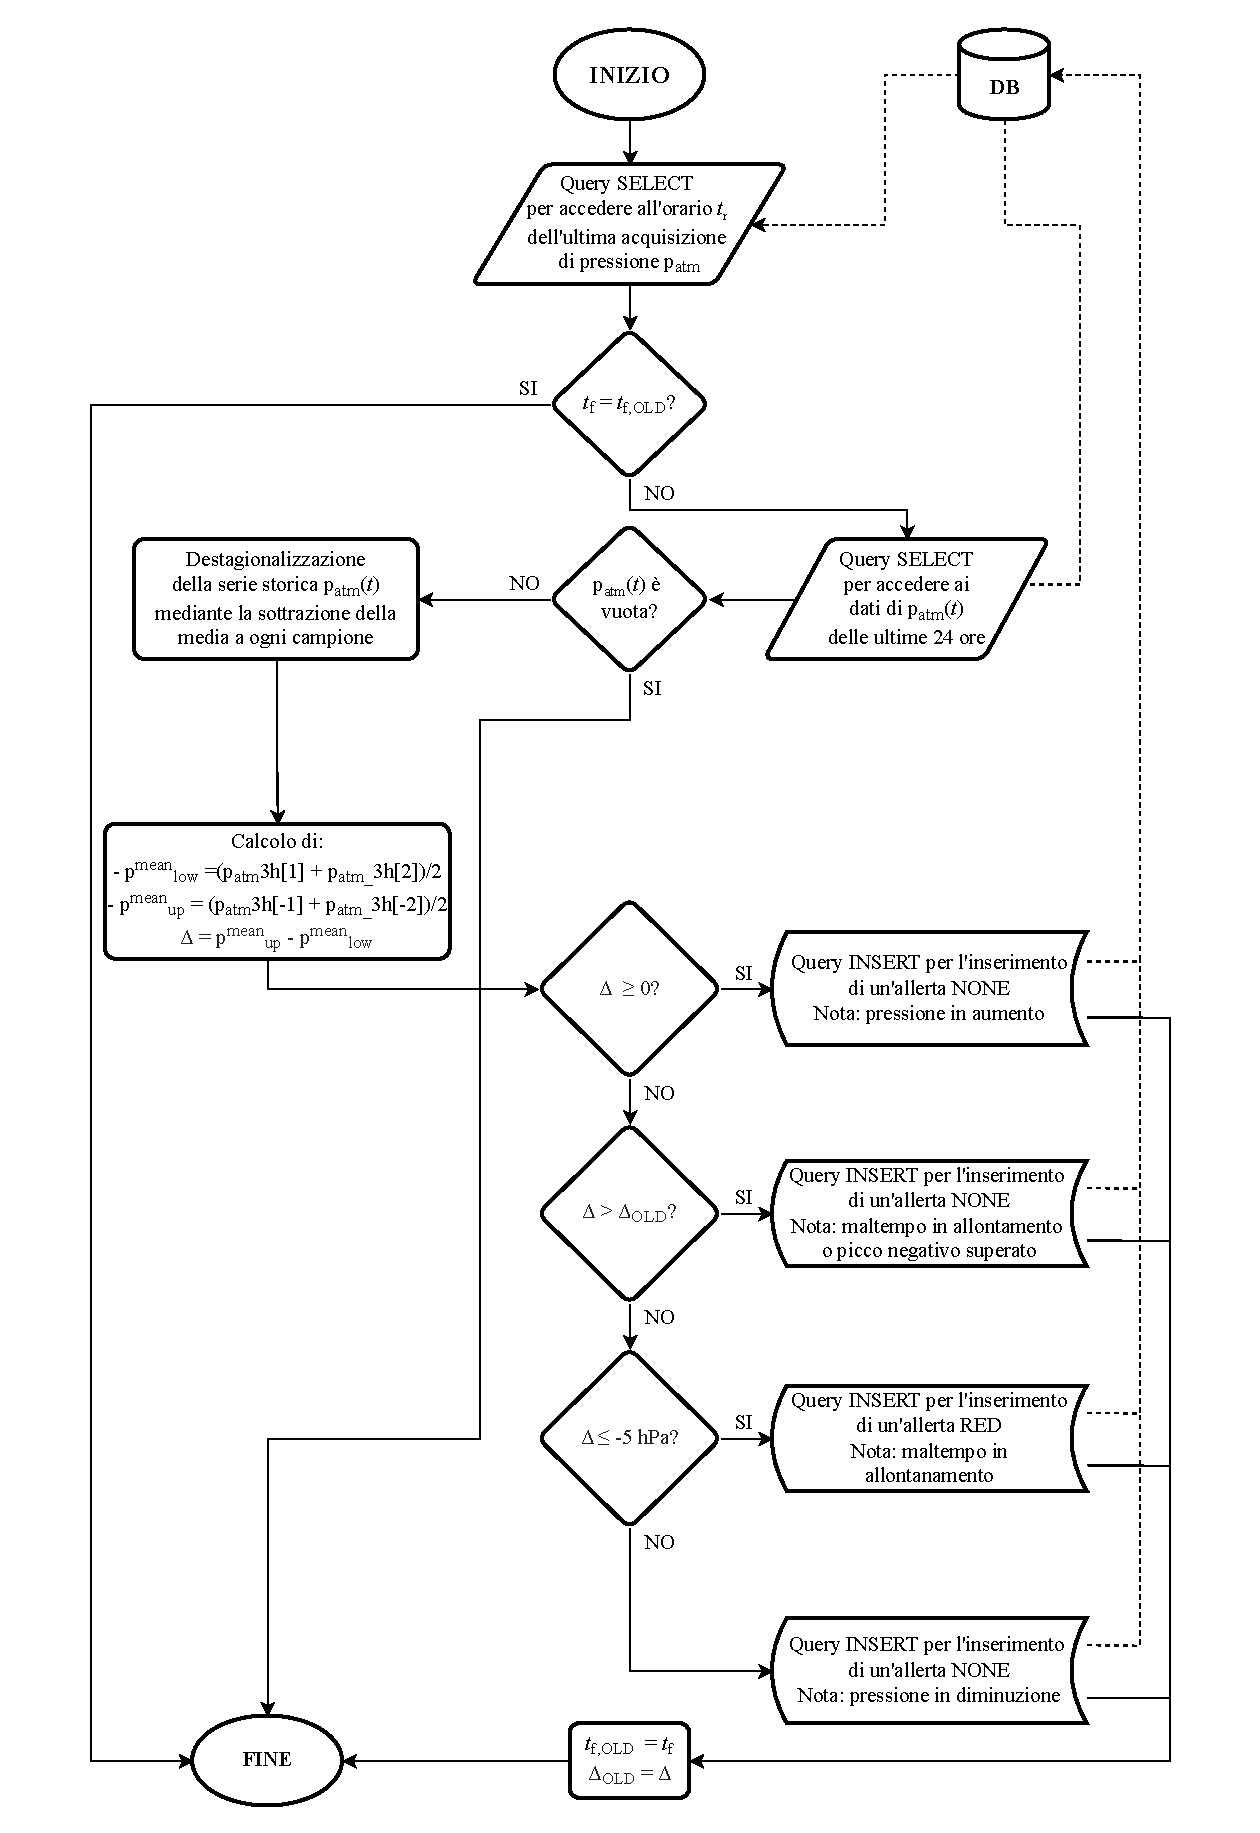
\includegraphics[height=590px]{./Iterazione 3/OtherFiles/FC - Generatore allerte BW.pdf}
	\caption{Diagramma di flusso relativo all'algoritmo di generazione delle allerte maltempo.}
	\label{fig:BFFlowChart}
\end{figure}

\clearpage

\paragraph{Generatore di allerte nebbia e brina}

\subparagraph{Cenni di meteorologia} Per prevedere le formazioni di nebbia e brina è necessario calcolare il \textit{punto di rugiada} T$_d$, ossia la temperatura alla quale l'acqua contenuta nell'aria di un ambiente condensa e si trasforma in gocce d'acqua; esso viene raggiunto quando l'umidità relativa raggiunge il \SI{100}{\percent}, cioè nell'istante in cui l'aria diventa satura e non riesce più a contenere l'umidità ambientale. Il punto di rugiada si determina tramite l'\textit{approssimazione di Magnus-Tetens}:
\[ T_d = \frac{b \cdot \alpha(T,UR)}{a - \alpha(T,UR)}\]
\[\mbox{con } \alpha(T,UR) = \frac{a \cdot T}{b + T} + \ln(UR) \mbox{, } a = \si{17,27} \mbox{ e } b = \si{237,7}\si{\degreeCelsius}\]
\[T\mbox{ (temperatura misurata): } \SI{-20}{\degreeCelsius} < T < \SI{60}{\degreeCelsius}\]
\[UR\mbox{ (umidità relativa): } 0,01 < UR < 1,00\]
La nebbia si forma quando T = T$_d$, mentre la brina quando T = T$_d$ con T$_d < 0$

\subparagraph{Descrizione dell'algoritmo} Per generare le allerte nebbia e brina si deve calcolare la temperatura di rugiada T$_d$ (o \textit{dew point}), la quale dipende della temperatura T e dell'umidità relativa UR. Dopo aver verificato che i dati non siano già stati analizzati ($t_f \neq t_{f,OLD}$), il primo passo dell'algoritmo (\Fig\ref{fig:FFFlowChart1}) consiste nell'eseguire una query per accedere ai dati di temperatura delle ultime 24 ore rilevati dalla stazione APRS.FI associata alla zona di riferimento del thread. Per effettuare una previsione della temperatura si è scelto l'utilizzo di un modello ARIMA, che permette anche di rendere stazionaria, se già non lo fosse, la serie storica tramite differenziazioni. Per identificare il modello, ossia per stimare il valore dei suoi parametri a massima verosimiglianza (o MLE) e per svolgere l'analisi di complessità (una procedura basata sulla minimizzazione dell'indicatore AIC) è stata utilizzata la funzione \textit{auto\_arima} del modulo \textit{pmdarima} disponibile per in Python. A ogni iterazione dell'algoritmo viene stimato un nuovo modello utilizzando anche l'acquisizione più recente presente nel DB. Una volta conclusa l'operazione di stima del modello ARIMA, esso viene utilizzato per svolgere una predizione a 3 passi della temperatura, ossia a:
\begin{itemize}
	\item $t_1 = t_f + k$; 
	\item $t_2 = t_f + 2 \cdot k$;
	\item $t_3 = t_f + 3 \cdot k$; 
\end{itemize}
con \textit{k} che rappresenta il tempo che intercorre tra due rilevazioni consecutive da parte della stazione meteorologica (circa \SI{10}{\minute}) e $t_f$ la data e l'ora dell'acquisizione più recente presente nel DB. Lo stesso studio a scopo predittivo viene fatto anche per l'umidità relativa. Una volta note le previsioni di T e UR, esse vengono combinate per effettuare la predizione a 3 passi della temperatura di rugiada T$_d$. Dopodiché, vengono calcolati gli intervalli di validità I, IC$_1$, IC$_2$ e IC$_3$ entro i quali la temperatura deve rientrare affinché venga generata un'allerta. Essi sono necessari non solo perché non si otterrà mai un'uguaglianza precisa tra T(\textit{t}) e T$_d$(\textit{t}) a causa degli errori di predizione, ma anche perché la condensazione dell'acqua contenuta nell'aria può avvenire a una temperatura superiore a quella di rugiada; infatti, T$_d$ non tiene conto nè della temperatura del suolo, il quale potrebbe essere più freddo della colonna d'aria che lo sovrasta, nè della presenza di sostanze chimiche capaci di alterare il dew point. Gli intervalli sono asimmetrici poiché T non può essere più piccola di T$_d$; se così fosse l'umidità relativa supererebbe il \SI{100}{\percent}, un evento fisicamente impossibile. Per i criteri di generazione delle allerte si faccia riferimento alla figura \ref{fig:FFFlowChart2}. Si noti che l'allerta brina viene creata quando la temperatura, attuale $T(t_f)$ o prevista $\hat{T}(t_1|t_f)$, $\hat{T}(t_2|t_f)$ e $\hat{T}(t_3|t_f)$: 
\begin{itemize}
	\item rientra nel proprio intervallo di validità (es. $\hat{T}(t_1|t_f) \in$ IC$_1$ $= [\hat{T_d}(t_1|t_f);\hat{T_d}(t_1|t_f) + \SI{0.45}{\degreeCelsius}]$);
	\item è non-positiva (es. $\hat{T}(t_1|t_f) \le 0$).
\end{itemize} L'algoritmo, infine, termina con l'aggiornamento di $t_{f,OLD}$.        

\begin{figure}[h!]
	\centering
	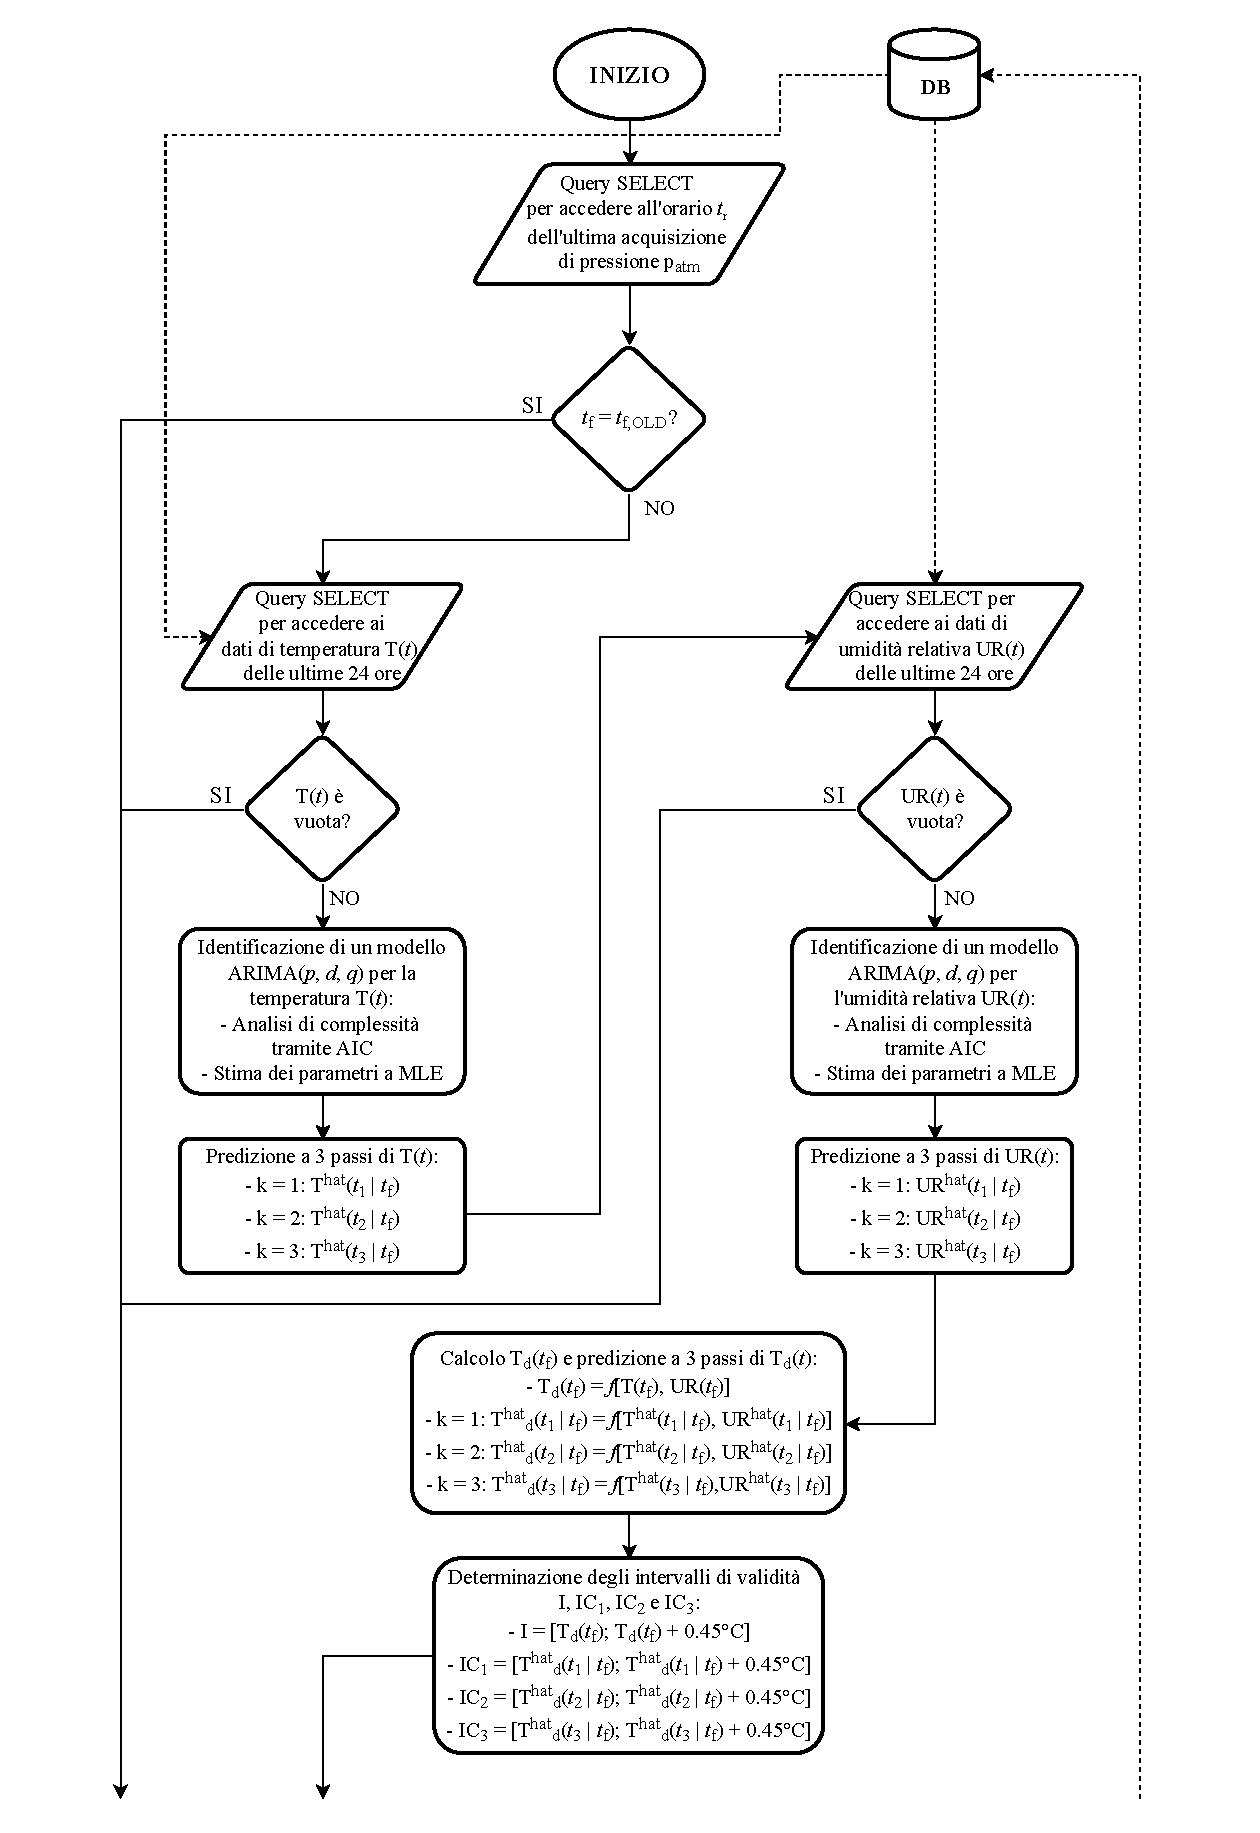
\includegraphics[height=590px]{./Iterazione 3/OtherFiles/FC - Generatore allerte F&F(1).pdf}
	\caption{Diagramma di flusso relativo all'algoritmo di generazione delle allerte nebbia e brina, prima parte.}
	\label{fig:FFFlowChart1}
\end{figure}

\begin{figure}[h!]
	\centering
	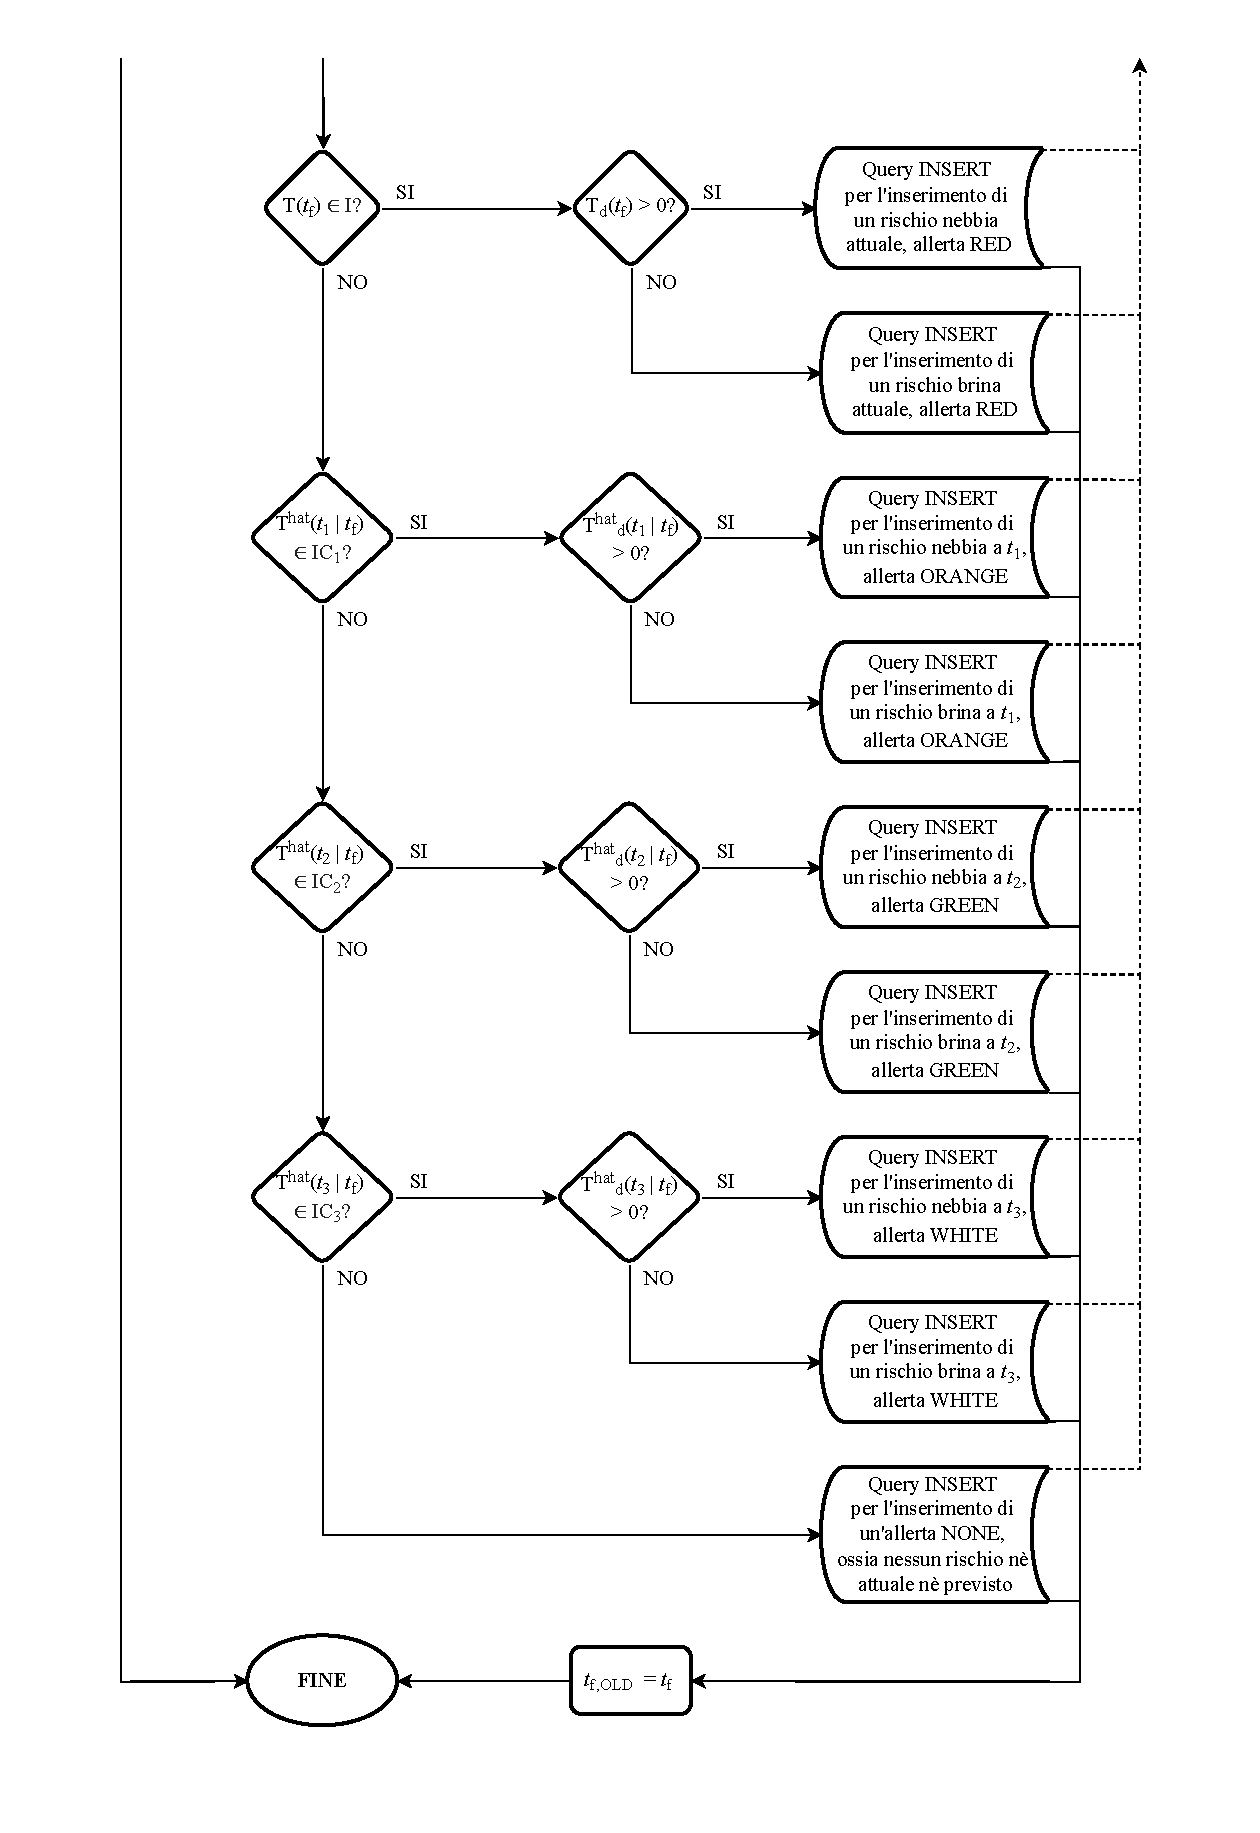
\includegraphics[height=590px]{./Iterazione 3/OtherFiles/FC - Generatore allerte F&F(2).pdf}
	\caption{Diagramma di flusso relativo all'algoritmo di generazione delle allerte nebbia e brina, seconda parte.}
	\label{fig:FFFlowChart2}
\end{figure}

\clearpage

\subsection{Algoritmo}
Di seguito sono riportati gli pseudocodici dell'algoritmo e delle funzioni alla base della generazione degli allarmi implementati nell'iterazione 3 e già descritti tramite i diagrammi di flusso presentati precedentemente.

\SetKwComment{Comment}{/* }{ */}
\RestyleAlgo{ruled}
\begin{algorithm}
	\caption{Data Analyzer}
	\SetKwProg{Al}{algoritmo}{ is}{end}
	\Al{generateAlarms($area\_DS$, $num\_areas$)}{
		\textbf{/* Avvio dei generatori di allerte */}\;
		\For{$i = 1$ \KwTo $num\_areas$}{
			\underline{badWeatherAlertsCreator}($area\_DS$ [$i$ ; `nameAprStation'], $area\_DS$[$i$ ; `idArea'], $i$, $old\_final\_time\_list$, $old\_delta\_list$)\;
			\underline{fogFrostAlertsCreator}($area\_DS$ [$i$ ; `nameAprStation'], $area\_DS$[$i$ ; `idArea'], $i$, $old\_final\_time\_list$)\;
		}
	}
\label{alg:1}
\end{algorithm}

\begin{algorithm}
	\SetKwProg{Fn}{function}{ is}{end}
	\SetKwProg{Class}{Class}{:}{end}
	\SetKwIF{If}{ElseIf}{Else}{if}{then}{else if}{else}{end}
	\caption{generatore di allerte maltempo}
	\Fn{badWeatherAlertsCreator(station\_code, areaID, index, old\_final\_time\_list, old\_delta\_list)}{
		$recent\_time \gets$ data ultima acquisizione della stazione $station\_code$\;
		\textbf{/* Interruzione della funzione se non ci fosse una nuova acquisizione */}\;
		\If{$recent\_time = old\_final\_time\_list\left[index\right]$}{
			\textbf{exit}\;
		}
		\textbf{/* Elaborazione della serie storica relativa alla pressione atmosferica */}\;
		$pressure\_DS\gets$ recupera i dati di pressione atmosferica delle ultime \num{24} ore della stazione $station\_code$\;
		\If{$parameter\_DS$ is empty}{\textbf{exit}\;}
		$p\_mean \gets$ mean($pressure\_DS$)\;
		\For{$i = 1$ \KwTo lenght($pressure\_DS$)}{
			$pressure\_DS$[$i$] $\gets pressure\_DS$[$i$] - $p\_mean$ \Comment*[r]{Destagionalizzazione} 
		}
		$pressure\_DS \gets$ seleziona pressione ultime \num{3} ore di $pressure\_DS$\;
		$p\_low \gets$ mean($pressure\_DS$[\num{1}:\num{2}])\;
		$p\_up \gets$ mean($pressure\_DS$[end-\num{1}:end])\;
		$delta \gets p\_up - p\_low$\;
		\textbf{/* Generazione delle allerte relative al maltempo */}\;
		\uIf{$delta \ge 0$}{
			crea un'allerta NONE, pressione in aumento\;
			inserisci l'allerta nel DB\;
		}
		\uElseIf{$delta > old\_delta\_list\left[index\right]$}{
			crea un'allerta NONE, maltempo in allontanamento\;
			inserisci l'allerta nel DB\;
		}
		\uElseIf{$delta < -\SI{5}{\hecto\pascal}$}{
			crea un'allerta RED, maltempo in avvicinamento\textbackslash picco negativo superato\;
			inserisci l'allerta nel DB\;
		}
		\Else{
			crea un'allerta NONE, pressione in diminuzione\;
			inserisci l'allerta nel DB\;
		}
		\textbf{/* Aggiornamento delle strutture dati di supporto */}\;
		$old\_final\_time\_list \left[index\right] \gets recent\_time$\;
		$old\_delta\_list\left[index\right] \gets delta$\;
	}
\label{alg:2}
\end{algorithm}

\begin{algorithm}
	\SetKwProg{Fn}{function}{ is}{end}
	\SetKwIF{If}{ElseIf}{Else}{if}{then}{else if}{else}{end}
	\caption{generatore di allerte nebbia e brina, parte 1}
	\Fn{fogFrostAlertsCreator(station\_code, areaID, index, old\_final\_time\_list)}{
		$recent\_time \gets$ data ultima acquisizione della stazione $station\_code$\;
		\textbf{/* Interruzione della funzione se non ci fosse una nuova acquisizione */}\;
		\If{$recent\_time = old\_final\_time\_list\left[index\right]$}{
			\textbf{exit}\;
		}
		\textbf{/* Predizione dei valori di temperatura e umidità relativa */}\;
		$summaryT \gets$ crea una tabella per la temperatura con colonne \{`I\_low', `value', `I\_up'\} e righe \{`tf', `t1', `t2', `t3'\}\;
		$summaryUR \gets$ crea una tabella per l'umidità relativa con colonne \{`I\_low', `value', `I\_up'\} e righe \{`tf', `t1', `t2', `t3'\}\;
		$summaryTd \gets$ crea una tabella per la temperatura di rugiada con colonne  \{`I\_low', `value', `I\_up'\} e righe \{`tf', `t1', `t2', `t3'\}\;
		\underline{tempURForecaster}(`temperature',$station\_code$, $summaryT$)\;
		\underline{tempURForecaster}(`umidity', $station\_code$, $summaryUR$)\;
		\textbf{/* Calcolo dei valori attuali e previsti della temperatura di rugiada */}\;

		\For{$i$ \KwTo $summaryTd.rows$}{
			$summaryTd$[$i$ ; `value'] $\gets$ calcolo temperatura di rugiada usando $summaryT$[$i$,`value'] e $summaryUR$[$i$,`value']\;
			$summaryTd$[$i$ ; `I\_up'] $\gets$ $summaryTd$[$i$ ; `value'] + \num{0.45}\;
			$summaryTd$[$i$ ; `I\_low'] $\gets$ $summaryTd$[$i$ ; `value']\;
		}
		\textbf{/* Generazione delle allerte nebbia e brina */}\;
		\underline{alertsCreator}($summaryT$, $summaryTd$)\;
		$old\_final\_time\_list \left[index\right] \gets recent\_time$\;
	}
\label{alg:3}
\end{algorithm}

\begin{algorithm}
	\SetKwProg{Fn}{function}{ is}{end}
	\SetKwIF{If}{ElseIf}{Else}{if}{then}{else if}{else}{end}
	\caption{generatore di allerte nebbia e brina, parte 2}
	\Fn{tempURForecaster(parameter, station\_code, dataToUpdate)}{
		\eIf{$parameter$ = `temperature'}{
			$parameter\_DS \gets$ recupera dati di temperatura delle ultime \num{24} della stazione $station\_code$\;
		}{
			$parameter\_DS \gets$ recupera dati di umidità delle ultime \num{24} della stazione $station\_code$\;
		}
		
		\If{$parameter\_DS$ is empty}{\textbf{exit}\;}
		
		\textbf{/* Analisi dei dati */}\;
		$model \gets$ fitARIMA($parameter\_DS$[all ; $parameter$], $start\_complexity$ = [\num{1}, \num{1}, \num{1}], $stop\_complexity$ = [\num{3}, \num{3}, \num{3}]) \Comment*[r]{Stima del modello ARIMA}
		$k \gets$ \num{3} \Comment*[r]{Passo della predizione}
		$\left[fc, confint \right] \gets$ predict($model$, $k$) \Comment*[r]{Predizione a $k$ passi}
		\textbf{/* Aggiornamento del dataset */}\;
		$dataToUpdate$[`tf' ; all] $\gets$ $parameter\_DS$[end ; $parameter$]\;
	
		\For{$i$ = 1 to k}{
			$dataToUpdate[$i$,'value'] \gets$ fc[i]\;
			$dataToUpdate[$i$,'I\_low'] \gets$ confint[i,'$ic\_low$']\;
			$dataToUpdate[$i$,'I\_up'] \gets$ confint[i, '$ic\_up$']\;
		}
	}
\label{alg:4}
\end{algorithm}

\begin{algorithm}
	\SetKwProg{Fn}{function}{ is}{end}
	\SetKwIF{If}{ElseIf}{Else}{if}{then}{else if}{else}{end}
	\caption{generatore di allerte nebbia e brina, parte 3}
	\Fn{alertsCreator(summaryT, summaryTd)}{
		\uIf{$summaryTd$ ['tf' ; 'I\_low'] $ \le summaryT$[`tf' ; `value']$ \le summaryTd$ [`tf' ; `I\_up']}{
			\eIf{$summaryT$[`tf' ; `value'] $>0$}{
				crea un rischio nebbia attuale, allerta RED\;
				inserisci l'allerta nel DB\;	
			}{
				crea un rischio brina attuale, allerta RED\;
				inserisci l'allerta nel DB\;	
			}
		}

		\uElseIf{ $summaryTd$[`t1' ; `I\_low']$\le summaryT$[`t1' ; `value'] $\le summaryTd$[`t1' ; `I\_up']}{
			\eIf{$summaryT$[`t1' ; `value'] $>0$}{
				crea un rischio nebbia tra \SI{10}{\minute}, allerta ORANGE\;
				inserisci tramite una query l'allerta nel DB\;
			}{
				crea un rischio brina tra \SI{10}{\minute}, allerta ORANGE\;
				inserisci tramite una query l'allerta nel DB\;
			}	
		}
		\uElseIf{$summaryTd$[`t2' ; `I\_low']$ \le summaryT$[`t2' ; `value']$\le summaryTd$[`t2' ; `I\_up']}{
			\eIf{$summaryT$[`t2' ; `value'] $>0$}{
				crea un rischio nebbia tra \SI{20}{\minute}, allerta GREEN\;
				inserisci tramite una query l'allerta nel DB\;
			}{
				crea un rischio brina tra \SI{20}{\minute}, allerta GREEN\;
				inserisci tramite una query l'allerta nel DB\;
			}
		}
		\uElseIf{$summaryTd$[`t3' ; `I\_low']$\le summaryT$[`t3' ; `value']$\le summaryTd$[`t3' ; `I\_up']}{
			\eIf{$summaryT$[`t3' ; `value'] $>0$}{
				crea un rischio nebbia tra \SI{30}{\minute}, allerta WHITE\;
				inserisci tramite una query l'allerta nel DB\;
			}{
				crea un rischio brina tra \SI{30}{\minute}, allerta WHITE\;
				inserisci tramite una query l'allerta nel DB\;
			}	
		}
		\Else{
			crea un'allerta NONE, nessun rischio nè attuale nè previsto\;
			inserisci tramite una query l'allerta nel DB\;
		}
	}
\label{alg:5}
\end{algorithm}

\clearpage

\paragraph{Analisi complessità}
Procediamo ora con l'analisi della complessità temporale dell'algoritmo. 

Nello psudocodice \Alg\ref{alg:1} è riportato l'entry point dell'algoritmo. Infatti, per ogni area vengono chiamate le funzioni \textit{badWeatherAlertsCreator} e \textit{fogFrostAlertsCreator} che si occupano della generazione delle allerte. Queste due funzioni avranno un costo costante per ogni area analizzata. Analizziamo più in dettaglio il costo computazionale delle funzioni:

\begin{itemize}
	\item \textbf{badWheatherAlertsCreator} (\Alg\ref{alg:2}): questa funzione genera un allarme se è in arrivo una perturbazione, analizzando la pressione atmosferica rilevata dalla stazione associata ad un area. Inizialmente, vengono effettuati dei controlli sui dati disponibili, analizzando con dei semplici costrutti \textit{if}, di costo costante in quanto basati su operazioni elementari di confronto, se i dati disponibili sono già stati analizzati oppure se non sono presenti dei dati nelle ultime 24 ore. Assumiamo che tipicamente questi controlli non determinino la terminazione della funzione, ossia che nel caso peggiore la computazione continui. Successivamente, è presente un ciclo for tramite cui viene effettuata la destagionalizzazione. Il ciclo for va da 1 a \textit{length(pressure\_DS)}. Tale parametro rappresenta il numero di valori di pressione delle ultime 24 ore di una particolare stazione e, poichè un nuovo valore di pressione viene inserito nel database ogni 10 minuti, tale parametro è mediamente costante e di conseguenza anche la complessità del ciclo risulta essere costante per ogni area. I restanti passaggi sono sequenze di operazioni elementari e costrutti \textit{if- then-else} che hanno una complessità temporale costante, poichè mutuamente esclusivi e composti da operazioni che possono essere considerate costanti in qualunque alternativa scelta.
	
	\item \textbf{fogFrostAlertsCreator} (\Alg\ref{alg:3}): questa funzione si occupa della generazione di allerte nebbia e brina, analizzando la temperatura e l'umidità relativa acquisita. Come nella funzione precedentemente descritta, se supponiamo di avere dati sufficienti a disposizione, la funzione esegue operazioni elementari di costo costante e, dal momento in cui viene chiamata una volta per ogni area, non contribuisce ad un aumento della complessità generale. In particolare si noti che la funzione utilizza i dati elaborati da tre sotto funzioni. Vengono effettuate due chiamate della funzione \textit{tempURForecaster} e una chiamata della funzione \textit{alertsCreator}. Le due funzioni sono descritte di seguito. Esse risultano avere complessità costante per ogni area analizzata.
	
	\item \textbf{tempURForecaster} (\Alg\ref{alg:4}): è la funzione principale dell'algoritmo, in cui vengono eseguite la stima del modello ARIMA e la predizione a k passi. Inizialmente, vengono recuperati o i dati di temperatura o di umidità della stazione scelta. Successivamente, come nelle funzioni precedenti, viene verificata la disponibilità di dati. Supponendo che tipicamente i dati siano presenti, e quindi riferendoci al caso peggiore, la computazione prosegue stimando il modello ARIMA e la predizione a tre passi della temperatura e umidità. \`E importante notare che il numero di parametri su cui vengono eseguite queste due operazioni è sempre lo stesso, perchè vengono presi i dati delle ultime 24 ore che sono costanti per ogni area e la predizione a tre passi può essere considerata costante per ogni modello stimato. Inoltre, la complessità del modello ARIMA stimato è stata limitata. Di conseguenza, queste operazioni possono essere considerate costanti per ogni area analizzata. Infine, il ciclo \textit{for} finale eseguirà sempre 3 iterazioni. Quindi, anche il costo di questa funzione è costante. 

	\item \textbf{alertsCreator} (\Alg\ref{alg:5}): questa funzione serve per inserire le allerte nebbia o brina nel database. Non sono presenti cicli, ma solo una sequenza di \textit{if-then-else} mutualmente esclusivi. Per ogni iterazione dell'algoritmo è possibile solamente eseguire una delle operazioni dei rami \textit{if-then-else}, il cui costo computazionale è costante.
\end{itemize}

Come si è potuto osservare, il costo totale dell'algortimo può essere considerato \textit{O(n\_areas)}, dove \textit{n\_areas} corrisponde al numero di aree inserite nel database e analizzate. Infatti, si è dimostrato come le due funzioni \textit{badWeatherAlertsCreator} e \textit{fogFrostAlertsCreator} abbiamo un costo costante per ogni area analizzata.

